\documentclass[10pt,a4paper]{article}
\usepackage[utf8]{inputenc}
\usepackage[english]{babel}
\usepackage{amsmath}
\usepackage{amsfonts}
\usepackage{amssymb}
\usepackage{graphicx}
\usepackage{minted}
% To use this package, you should have python version > 2.5 and pygments
% module installed.
\usepackage[left=2cm,right=2cm,top=2cm,bottom=2cm]{geometry}
\author{Arun Prasaad Gunasekaran}
\title{Cross Referencing}

\usepackage{natbib}
\bibliographystyle{apalike}

\begin{document}
\maketitle

\section{About this file}
This is an article for cross referencing tables, figures, equations, code snippets and bibliography entries.

\section{Cross-Reference Contents}

As mentioned Earlier, you have several cross referencing contents. Some of the important ones are:

\begin{itemize}
	\item Code Snippets
	\item Figures
	\item Tables
	\item Equations
	\item Bibliography Entries
\end{itemize}

\subsection{Images}
To put images, use the begin figure environment.

\begin{figure}
\centering
\fbox{
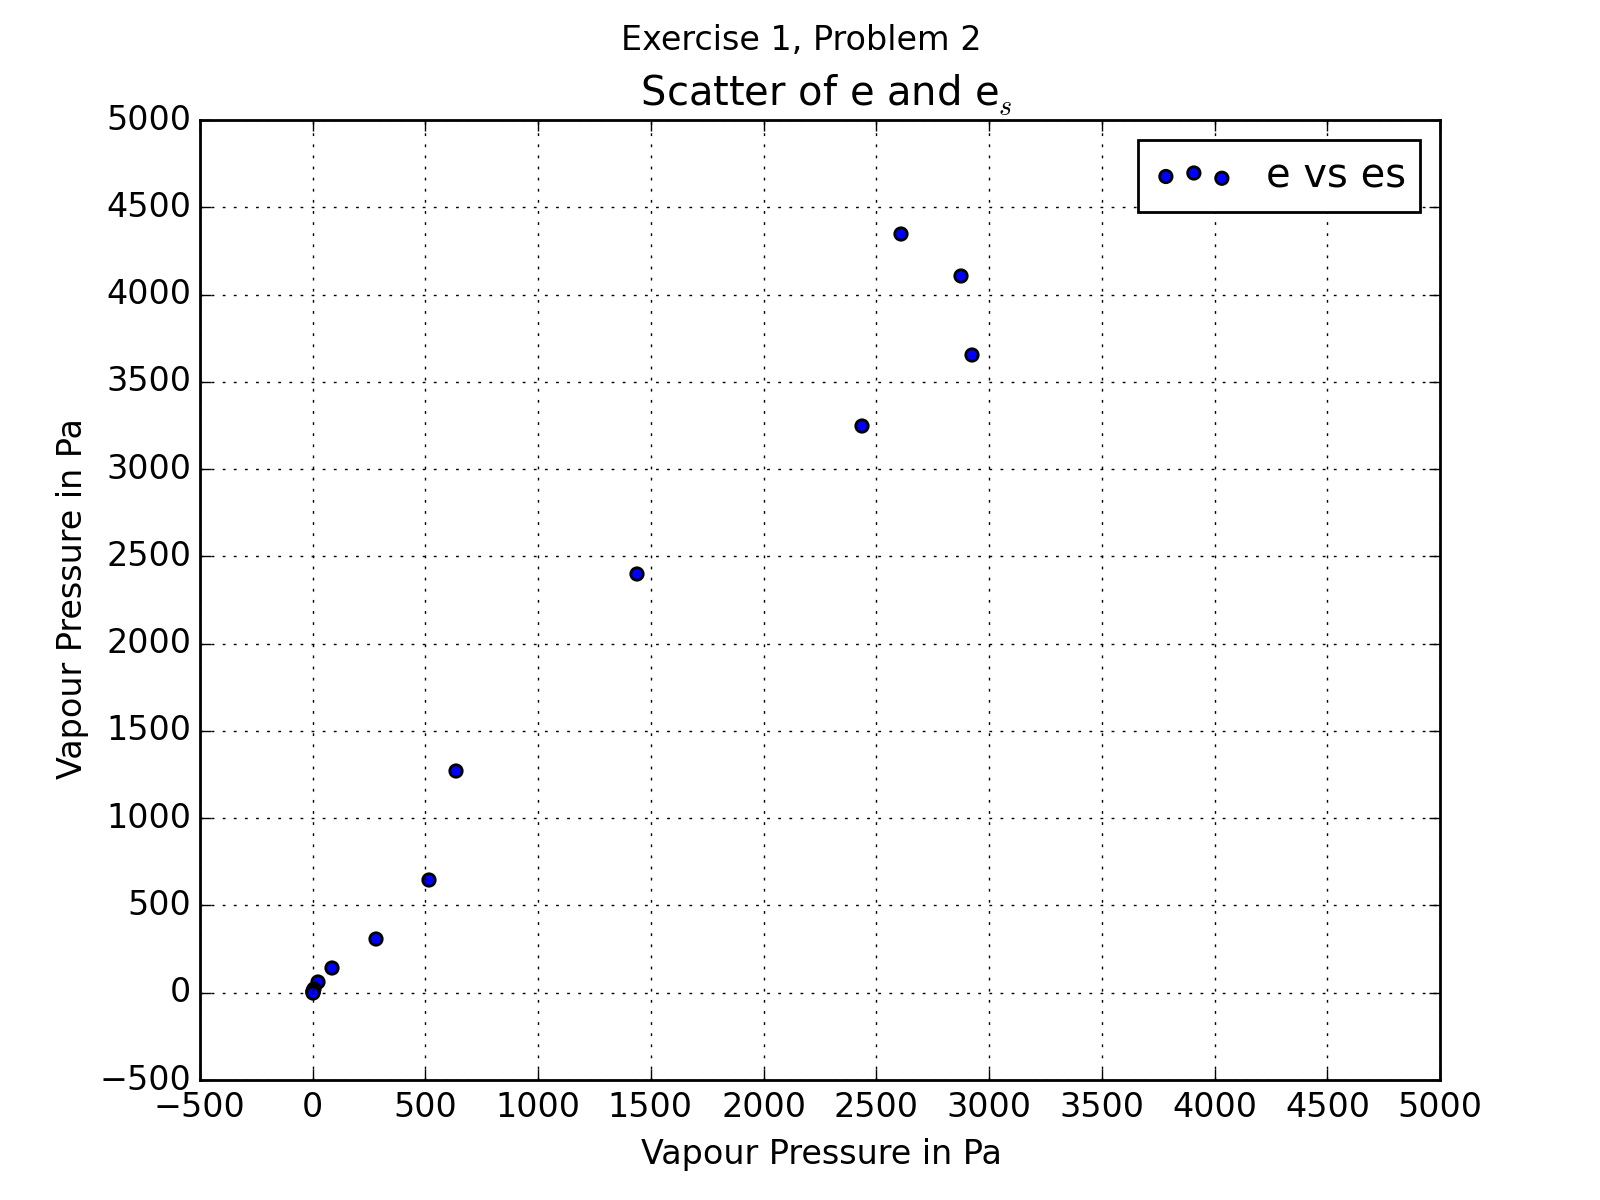
\includegraphics[scale=0.35]{eVSes.png}
}
\caption{The Scatter plot of E vs Es}
\label{eVSes}
\end{figure}

\begin{figure}
\centering
\fbox{
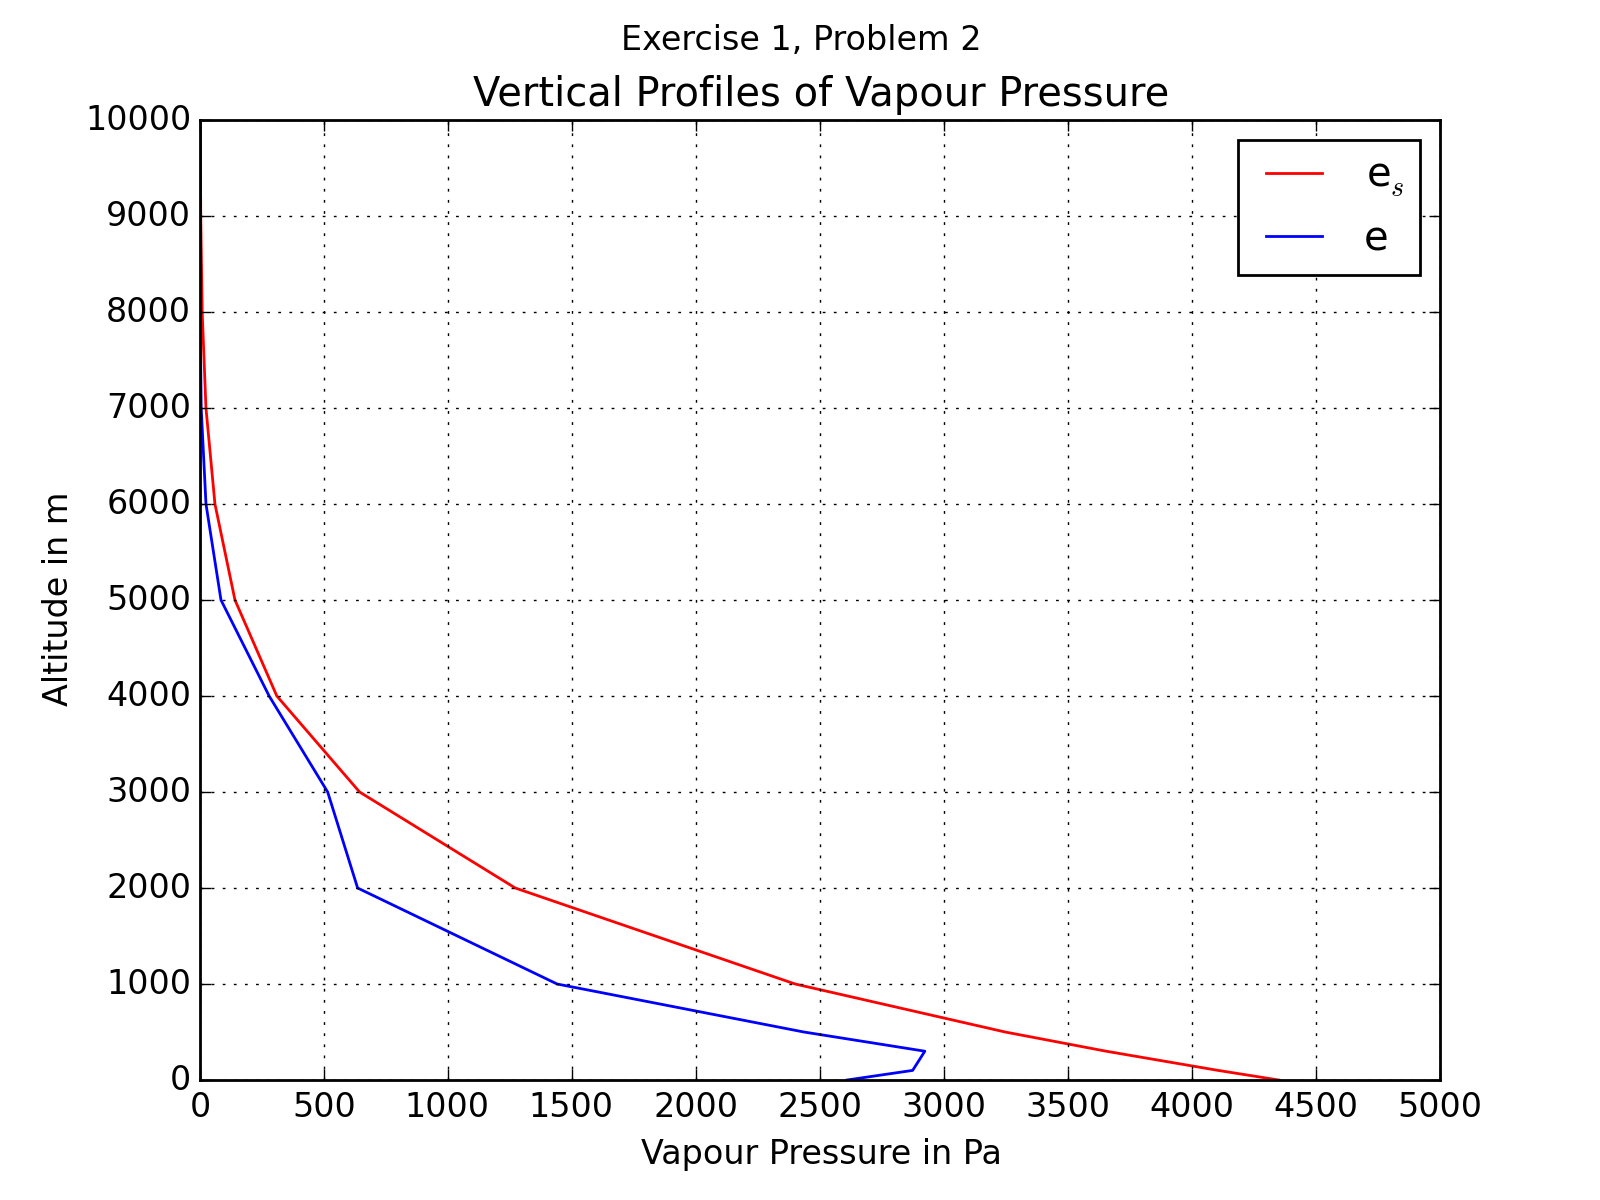
\includegraphics[scale=0.35]{eVsZ.png}
}
\caption{Vertical Profiles of E and ES}
\label{eVSz}
\end{figure}

\begin{figure}
\centering
\fbox{
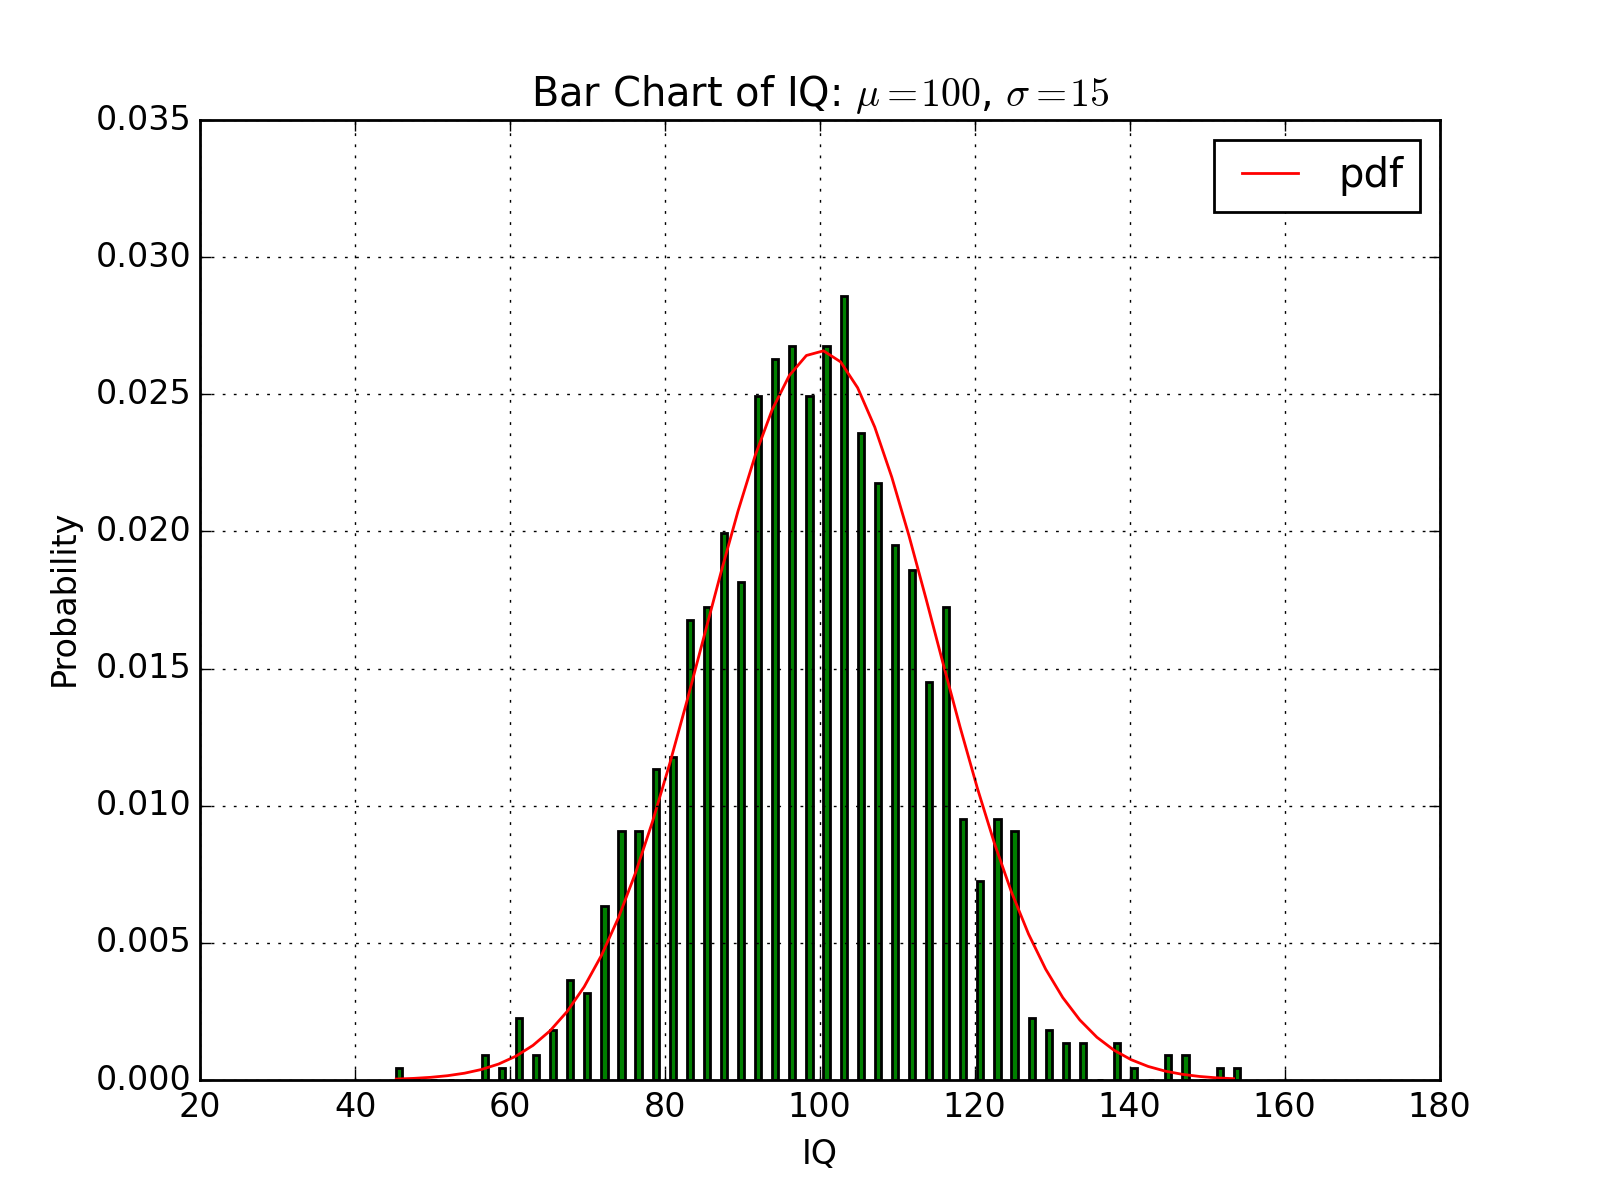
\includegraphics[scale=0.35]{IQ_bar.png}
}
\caption{Human IQ histobar}
\label{IQ}
\end{figure}

\subsection{Tables}

To put tables, use the table environment.

Table \ref{Tab1} has details of some houses in ASOIAF.

\begin{table}[h]
\centering
\caption{Exhaustive Details of Houses in ASOIAF}
\label{Tab1}
\begin{tabular}{|r|c|c|c|l|r|c|c|c|}
\hline
Sl.no & House & Kingdom & Sigil & Knightship & Leader & Weather & Origins & Capital \\\hline
1. & Stark & North & Direwolf & None & Eddard & Cold & First men & Winterfell\\\hline \hline
2. & Baratheon & Crownlands & Stag & Yes & Robert & Normal & Andals & King's Landing\\\hline
\end{tabular}
\end{table}

Table \ref{Tab2} has details of some houses in ASOIAF. Table \ref{Tab3} has details of some houses in ASOIAF.Table \ref{Tab1} has details of some houses in ASOIAF.

\begin{table}[h]
\centering
\caption{Few Details of Houses in ASOIAF}
\label{Tab2}
\begin{tabular}{|r|r|l|c|}
\hline
Sl.no & House & Kingdom & Sigil \\\hline
1. & Stark & North & Direwolf \\\hline
2. & Baratheon & Crownlands & Stag \\\hline
3. & Blackfyre & \multicolumn{2}{c|}{Not Applicable}\\\hline
4. & Targeryen & Valyria & Dragon\\
\cline{2-3}
 &  & Crownlands & \\ \hline 

\end{tabular}
\end{table}

\begin{table}
\centering
\caption{Few more Details of Houses in ASOIAF}
\label{Tab3}
\begin{tabular}{|c|c|c|c|c|}
\hline 
Sno & House & Leader & Captial & Sigil \\ 
\hline 
1 & Stark & Eddard & Winterfell & Direwolf \\ 
\hline 
2 & Martell & Doran & Dorne & Sun \\ 
\hline 
\end{tabular} 
\end{table}

\section{Code Snippets}

\begin{listing}
\begin{minted}[mathescape, linenos, numbersep=5pt, gobble=0, frame=lines, framesep=2mm]{c}
  // Program name : Circle_Area.C $ A = \pi r^2$
  /*
  Area of a circle will be explained here. Pi is $\pi$
  */
  
  int main()
  {
    const double pi = 3.1415926535;
    float r, A;
    
    printf("Enter the radius of the circle:");
    scanf("%f",&r );
    
    A = pi*r*r;
    
    printf("The Area of the circle with radius %f units is : %f units ", r, A);
   
    return 0;
   }

\end{minted}
\caption{A sample C code}
  \label{cs:1}
\end{listing}

\begin{listing}

\inputminted[mathescape, linenos, firstline=4, lastline=10, numbersep=5pt, gobble=0, frame=lines, framesep=2mm]{python}{ode_solve1.py}

\caption{A sample Python code}
  \label{cs:2}
\end{listing}

Code snippet \ref{cs:1} in page \pageref{cs:1} refers to the meta-data for a C# code. While Code snippet \ref{cs:2} in page \pageref{cs:2} refers to the meta-data for a Python code.

\bibliography{references}
\end{document}
